\chapter{Fire management basics}

\textbf{Prescribed fire operations are wildland fire operations.} 
\vspace{2em}

Despite being planned well in advance to achieve specific objectives within a defined period of time, conducting safe and effective prescribed fire operations requires all the attention to safety and communication of an emergency response. 
In fact, perhaps because of the planned, defined nature of such operations, it is even more critical to reinforce the duty each participant has to keep an eye out for themselves and each other. 

This chapter reviews some of the basic concepts for safety, leadership, and communication developed by the wildland fire community. 
While most of these concepts are presented within the context of wildfire suppression operations, almost all have relevance to prescribed fire, as well. 
And it is always important to ensure that members of the wildland fire community are on the same page and use common terminology, whether they are focused on putting fires out or starting them. 

\section{Situational Awareness}

A central concept in emergency management is \emph{situational awareness}, defined by the National Wildfire Coordinating Group as

\begin{quote}
	An on-going process of gathering information by observation and by communication with others. 
	This information is integrated to create an individual's perception of a given situation.\footnote{\href{https://www.nwcg.gov/term/glossary/situational-awareness-sa}{https://www.nwcg.gov/term/glossary/situational-awareness-sa}}
\end{quote}

The intention is to ensure the best possible understanding of a situation so that leaders can make safe tactical decisions and crew members can carry out tasks safely and effectively.
Thus, the on-going process of updating ones' understanding via communication and observation. 
Broadly speaking, the the goal is to increase \emph{decision space}\textemdash the room an individual has to consider necessary and available information before having to arrive at a decision. 
The converse of this idea is that poor situational awareness as a result of limited observation and communication often leads to hasty decisions. 

Situational awareness can be developed and practiced. 
One of the most effective ways to improve situational awareness is to gain experience in what factors merit focus, and which are distractions that ought to be filtered out. 

\section{LCES}

Critical to any safe operation is ensuring that the inputs necessary for situational awareness and contingency plans are in place. 
Four components of this safe operation space are Lookouts, Communications, Escape Routes, and Safety Zones (LCES; ~Fig.~\ref{fig:lces}). 

\begin{figure}
	\begin{center}
		
\includegraphics[width=1\columnwidth]
		{ops/lces_decal}
		%(Fig.~\ref{fig:lces})
	\end{center}
	\caption{The four aspects of LCES.
		\label{fig:lces}}
\end{figure}

Tactical decision-making requires current knowledge of the situation either through direct observation or communication with those who can directly observe critical parts of the operation space. 
Lookouts provide broad observations about personnel and the surrounding landscape and are especially important when 

Contingencies for safety include the capacity to get away from a bad situation, 

Think LCES is primarily a matter for wildfire suppression, where the lookouts are perched on mountaintops, crew bosses use radio repeaters, escape routes are marked with flagging, and bulldozers deliberately create safety zones?
Think again: 

	\begin{itemize}[noitemsep]	
	\item \textit{Lookouts:} A game trail prevented a backing fire from reaching a dry wetland at the bottom of a swale. 
	The burn boss wants someone to go down there and directly ignite it, but the torch operator would be unable to see crews on either fire line that low on the landscape. 
	The line boss assigns another crew member with a radio to go with the torch operator and maintain a position from which they can see both the torch operator and the line boss. 
	\emph{Crew members should rarely enter the burn unit and anyone in any proximity to unburned fuels should always have at least one person who ``has eyes on them'' who can anticipate and communicate changes in the fire environment.}
	\item \textit{Communication:} Bravo Crew is to begin the headfire operation only once Alpha Crew ties their line into a harvested field and has it at least 25 yards wide all the way across. 
	Although they can see the smoke plume working across the horizon, topography in the center of the burn unit prevents Bravo's line boss from seeing Alpha's firing team or the width of their blackline. 
	Bravo should not begin firing until Alpha has confirmed via radio that their tasks are complete. 
	\item \textit{Escape routes:} One side of the burn unit has a long, steep draw that has rocky outcroppings and low fuels that will prevent any fire from backing down the slope. 
	The burn boss wants the draw burned out to eliminate all fuels along the perimeter. 
	When they reach the mouth of the draw, instead of sending the primary torch around the bottom of the draw and out the other side, they instead take a UTV and two torches to the top of the draw and pull fire towards the mouth, so that all fire is moving up the draw away from them and into burned areas, such that at any point the crew can escape to the fire perimeter with fire at their back, rather than below and ahead of them. 
	\item \textit{Safety zones:} While mopping up along a mowed line, a crewmember makes sure to walk along the burned area, so that in case of a sudden wind shift they can step out of reach of the flames by retreating ``into the black.''
\end{itemize}

%\section{Common denominators} 
%
%\section{Driving safety} 
%\textbf{A R R I V E~~~A L I V E} 
%Always drive defensively.
%Reducing response vehicle speed
%can prevent rollovers.
%Red traffic signals and stop signs
%mean complete STOP.
%Insist that vehicle occupants use
%seat belts.
%Verify vehicle occupants are
%seated and belted.
%Evaluate road surface and
%weather conditions.
%Abide by federal and state motor
%vehicle laws.
%Lengthy response distances
%require frequent rest stops.
%Initiate standard vehicle backing operating procedures.
%Value occupant and public safety over time and speed.
%Enter dangerous curves and intersections cautiously.

%\newgeometry{textwidth=15cm}
\clearpage 
\section{Watch-out situations}		

\begin{minipage}{17cm}
	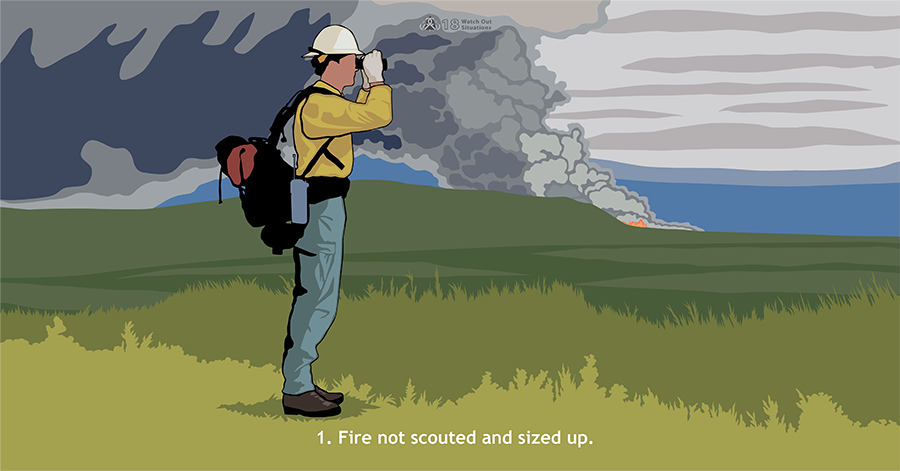
\includegraphics[width=0.49\textwidth, 
	trim={0cm 0cm 0cm 0cm}, 
	clip=true]
	{ops/pm118/118-01}
	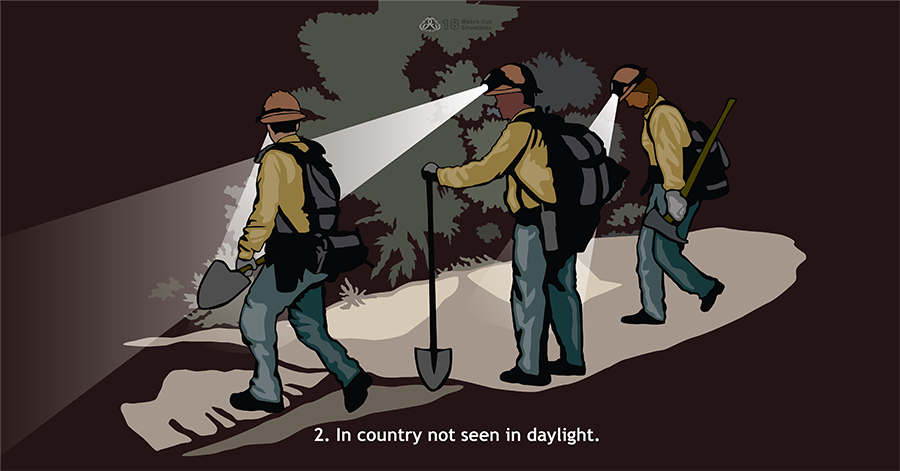
\includegraphics[width=0.49\textwidth, 
	trim={0cm 0cm 0cm 0cm}, 
	clip=true]
	{ops/pm118/118-02}  
	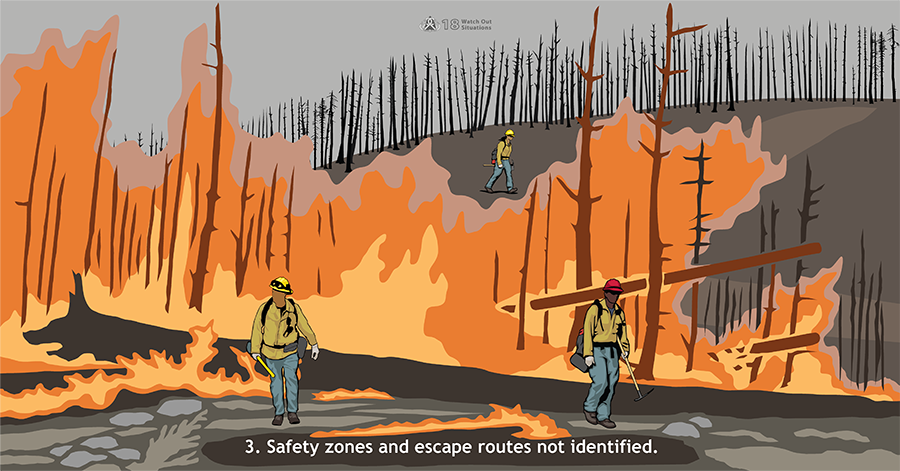
\includegraphics[width=0.49\textwidth, 
	trim={0cm 0cm 0cm 0cm}, 
	clip=true]
	{ops/pm118/118-03}
	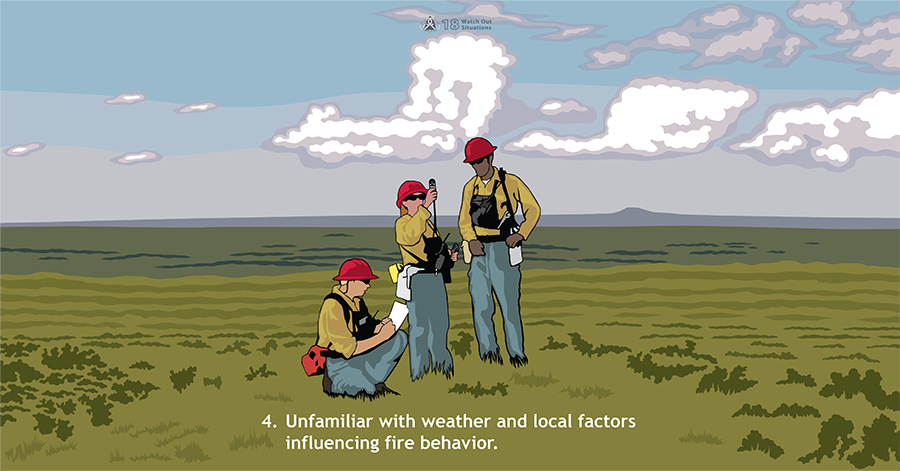
\includegraphics[width=0.49\textwidth, 
	trim={0cm 0cm 0cm 0cm}, 
	clip=true]
	{ops/pm118/118-04} 
		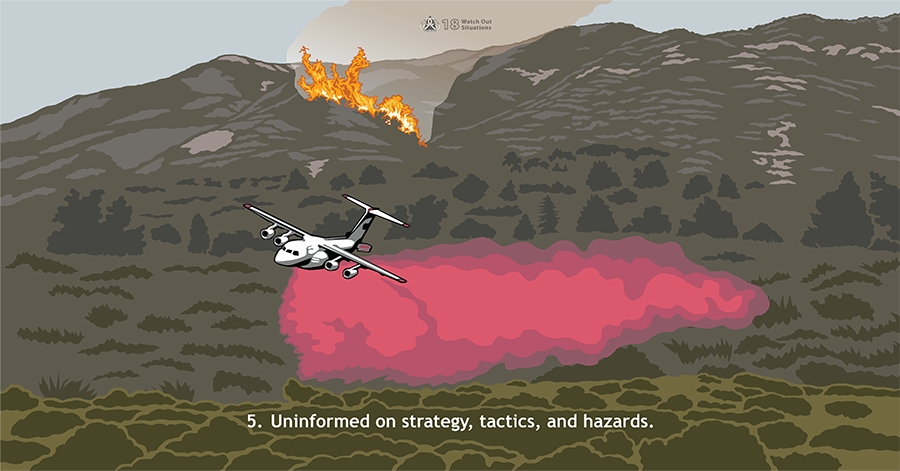
\includegraphics[width=0.49\textwidth, 
	trim={0cm 0cm 0cm 0cm}, 
	clip=true]
	{ops/pm118/118-05}
	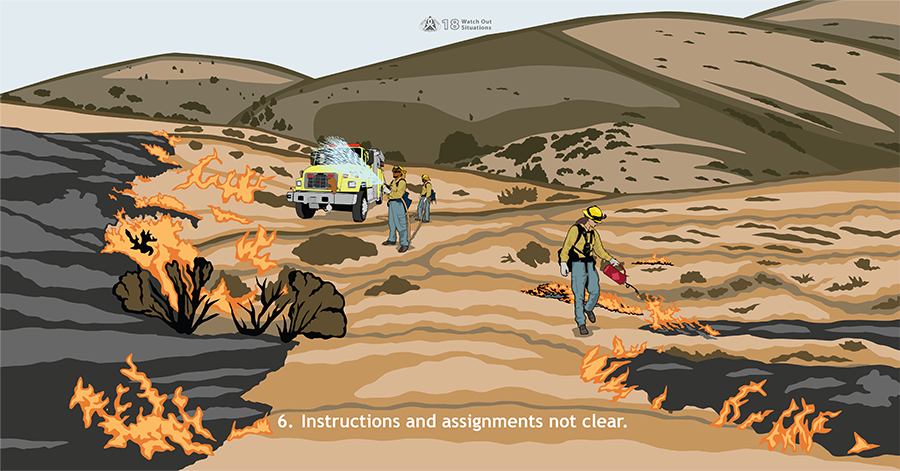
\includegraphics[width=0.49\textwidth, 
	trim={0cm 0cm 0cm 0cm}, 
	clip=true]
	{ops/pm118/118-06}  
	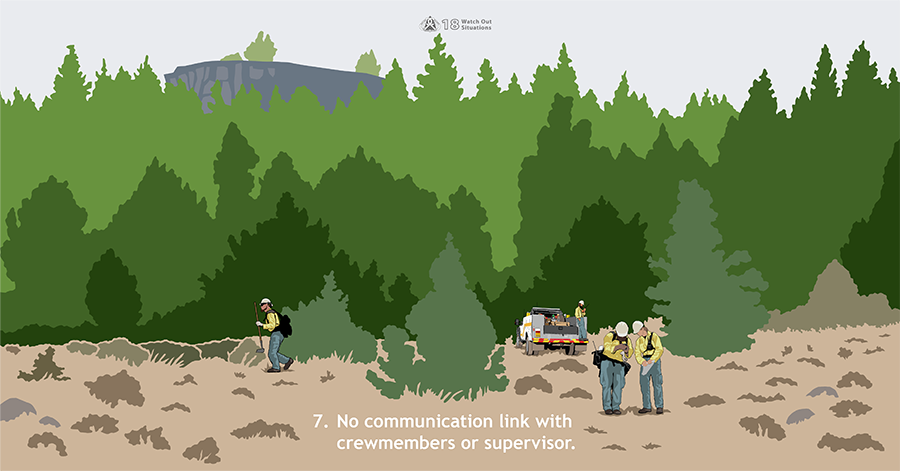
\includegraphics[width=0.49\textwidth, 
	trim={0cm 0cm 0cm 0cm}, 
	clip=true]
	{ops/pm118/118-07}
	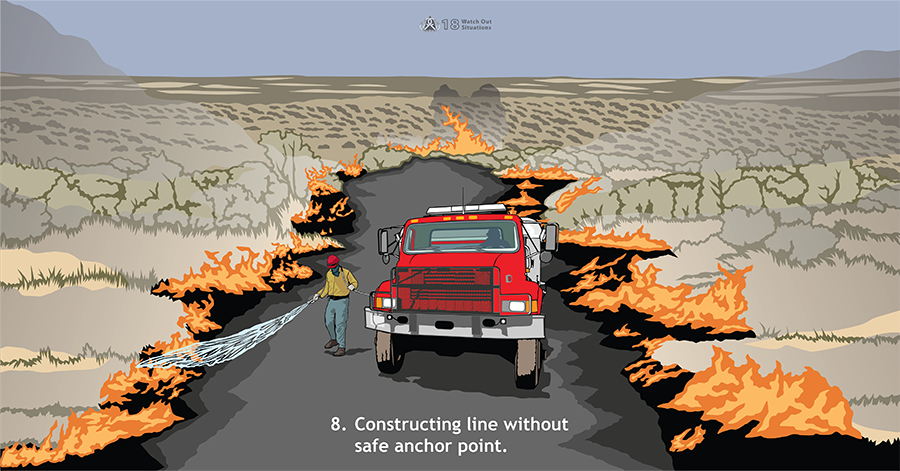
\includegraphics[width=0.49\textwidth, 
	trim={0cm 0cm 0cm 0cm}, 
	clip=true]
	{ops/pm118/118-08}  
		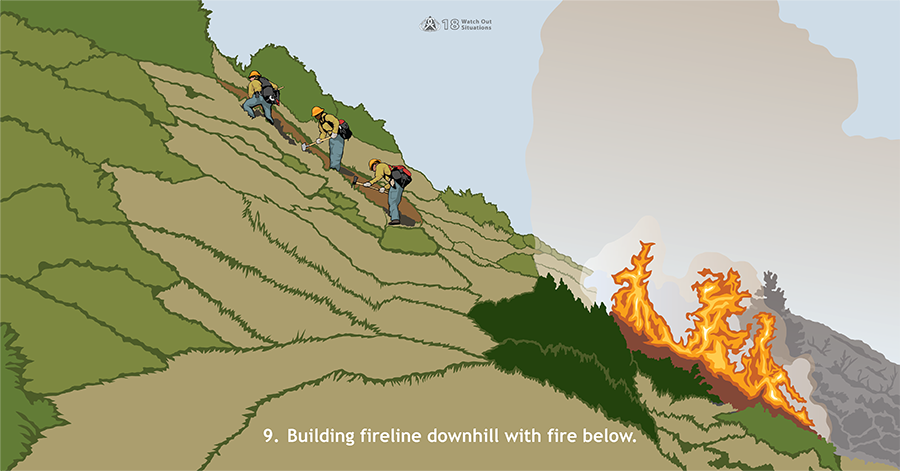
\includegraphics[width=0.49\textwidth, 
	trim={0cm 0cm 0cm 0cm}, 
	clip=true]
	{ops/pm118/118-09}
	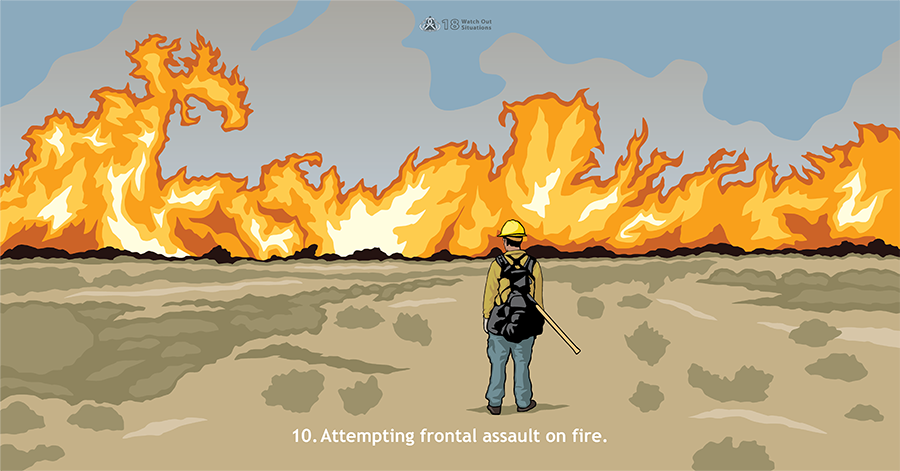
\includegraphics[width=0.49\textwidth, 
	trim={0cm 0cm 0cm 0cm}, 
	clip=true]
	{ops/pm118/118-10}  
\end{minipage}

\begin{minipage}{17cm}
	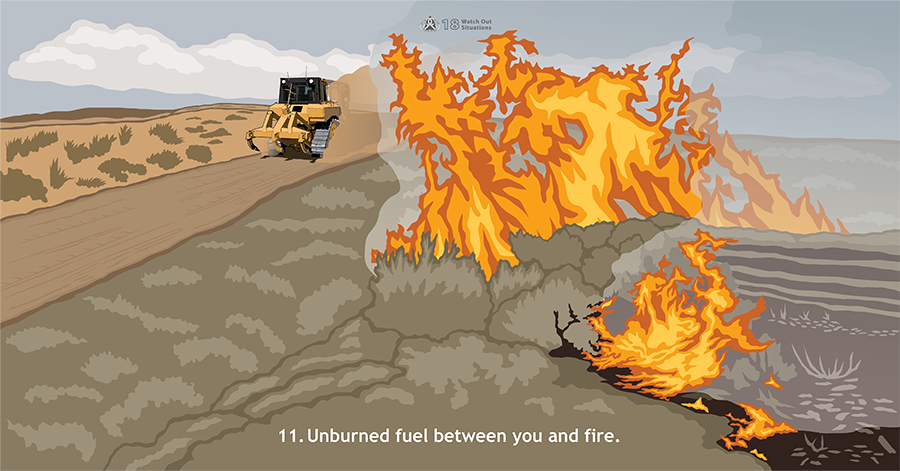
\includegraphics[width=0.49\textwidth, 
trim={0cm 0cm 0cm 0cm}, 
clip=true]
{ops/pm118/118-11}
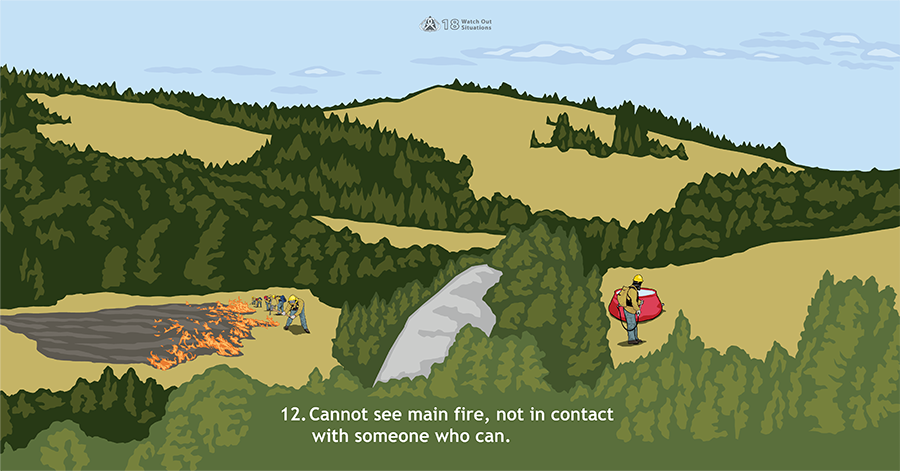
\includegraphics[width=0.49\textwidth, 
trim={0cm 0cm 0cm 0cm}, 
clip=true]
{ops/pm118/118-12} 
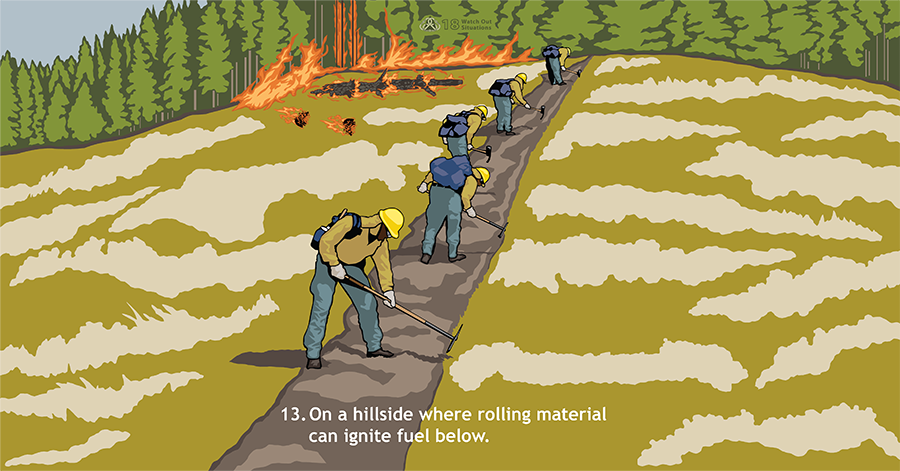
\includegraphics[width=0.49\textwidth, 
trim={0cm 0cm 0cm 0cm}, 
clip=true]
{ops/pm118/118-13}
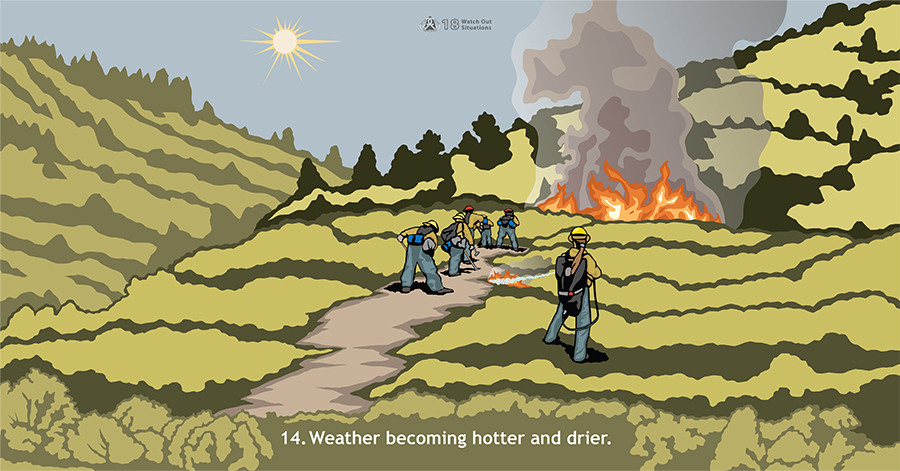
\includegraphics[width=0.49\textwidth, 
trim={0cm 0cm 0cm 0cm}, 
clip=true]
{ops/pm118/118-14}  
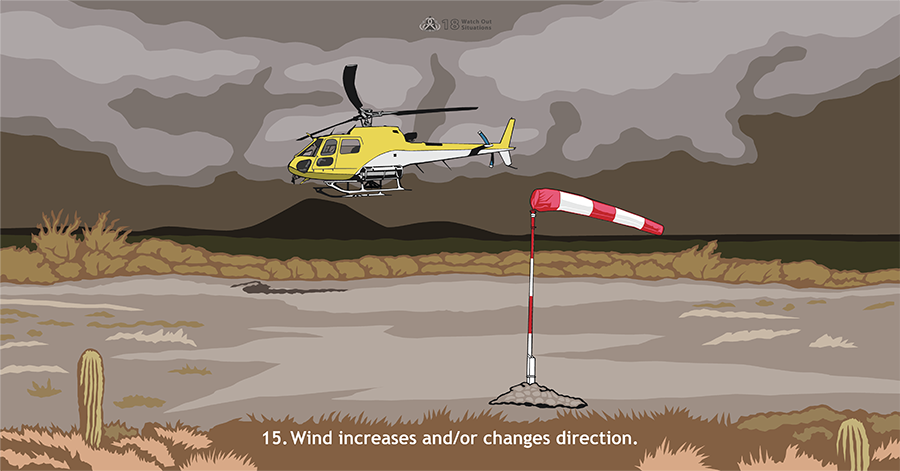
\includegraphics[width=0.49\textwidth, 
trim={0cm 0cm 0cm 0cm}, 
clip=true]
{ops/pm118/118-15}
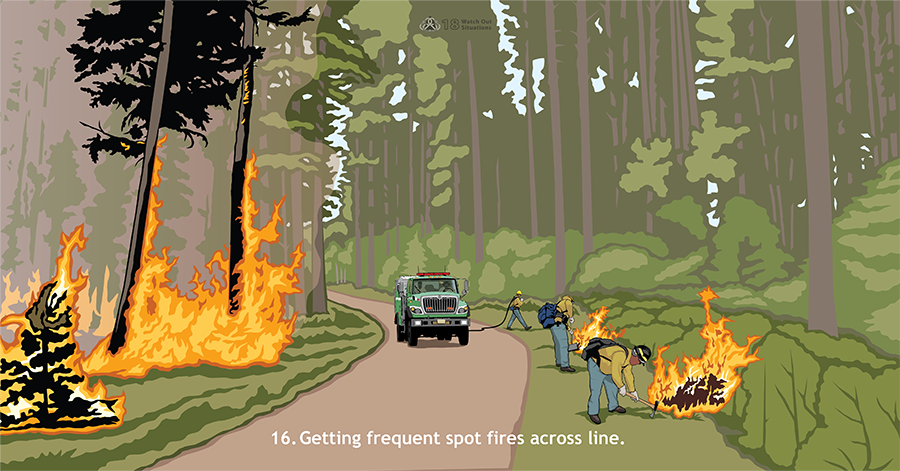
\includegraphics[width=0.49\textwidth, 
trim={0cm 0cm 0cm 0cm}, 
clip=true]
{ops/pm118/118-16} 
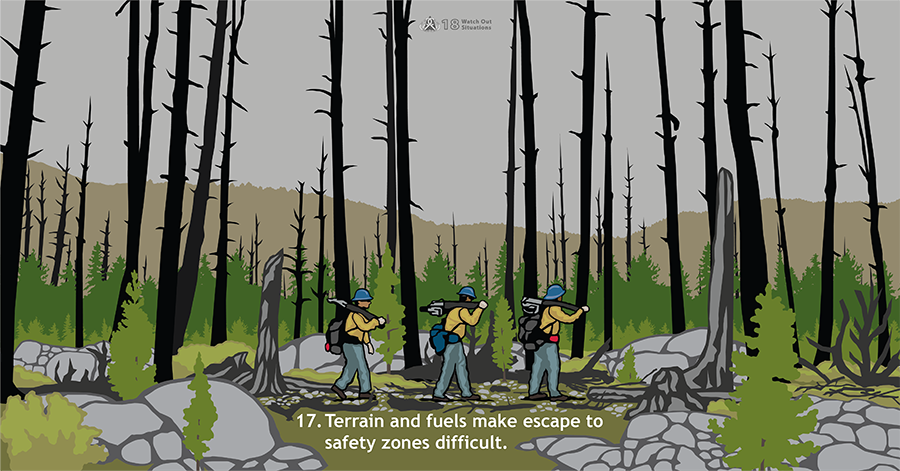
\includegraphics[width=0.49\textwidth, 
trim={0cm 0cm 0cm 0cm}, 
clip=true]
{ops/pm118/118-17}
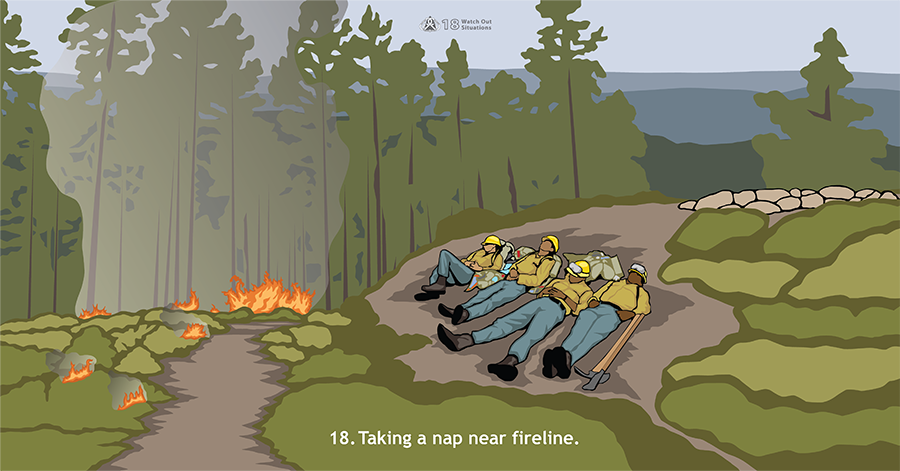
\includegraphics[width=0.49\textwidth, 
trim={0cm 0cm 0cm 0cm}, 
clip=true]
{ops/pm118/118-18}    

\end{minipage}

\section{Ten Standard Orders} 
\begin{minipage}{17cm}
	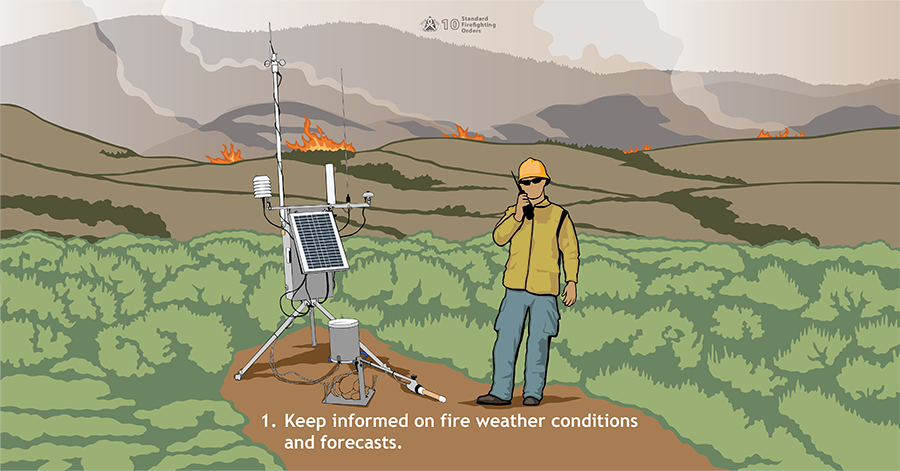
\includegraphics[width=0.49\textwidth, 
	trim={0cm 0cm 0cm 0cm}, 
	clip=true]
	{ops/pm110/110-01}
	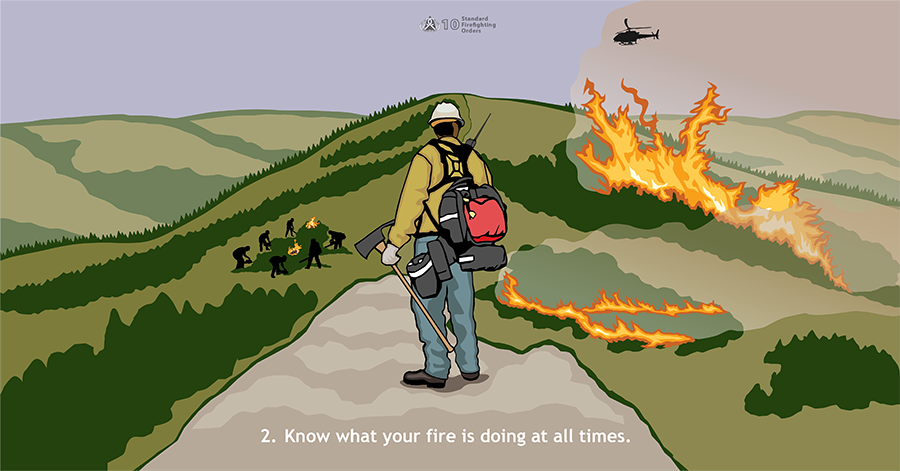
\includegraphics[width=0.49\textwidth, 
	trim={0cm 0cm 0cm 0cm}, 
	clip=true]
	{ops/pm110/110-02}	
	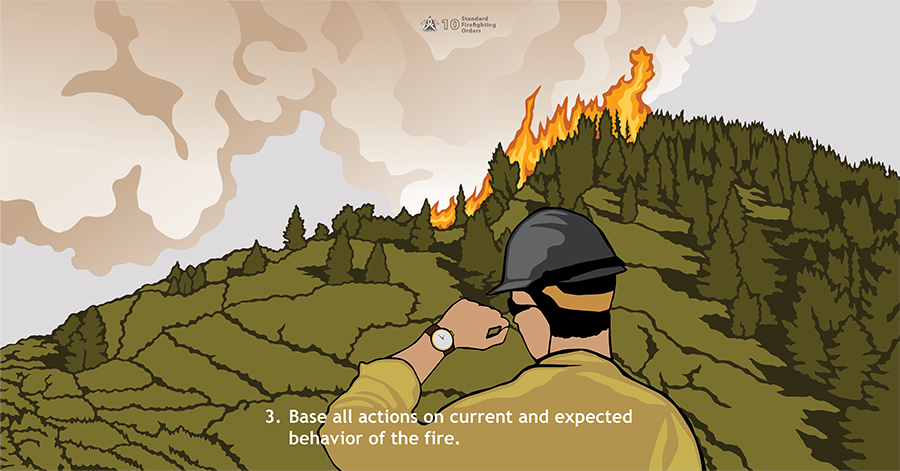
\includegraphics[width=0.49\textwidth, 
	trim={0cm 0cm 0cm 0cm}, 
	clip=true]
	{ops/pm110/110-03}
	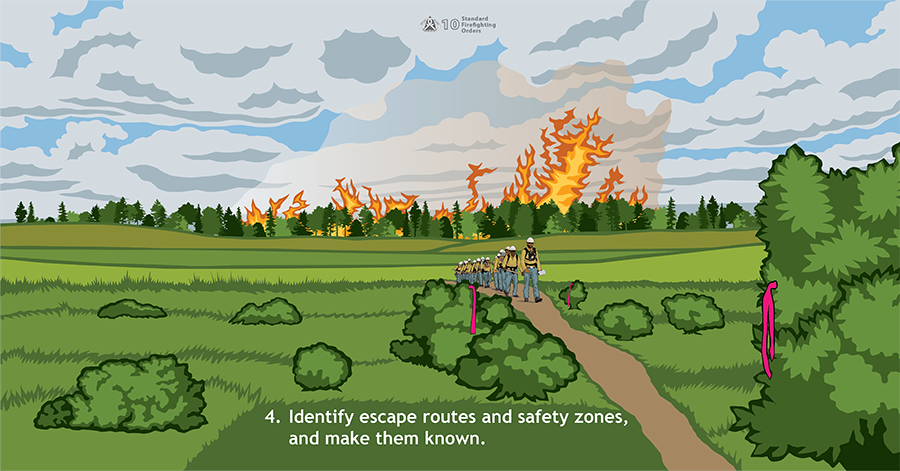
\includegraphics[width=0.49\textwidth, 
	trim={0cm 0cm 0cm 0cm}, 
	clip=true]
	{ops/pm110/110-04}	
	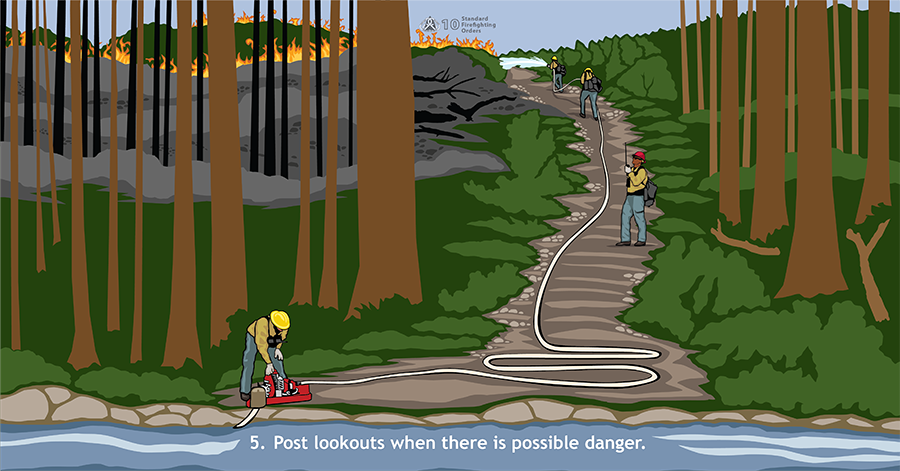
\includegraphics[width=0.49\textwidth, 
	trim={0cm 0cm 0cm 0cm}, 
	clip=true]
	{ops/pm110/110-05}
	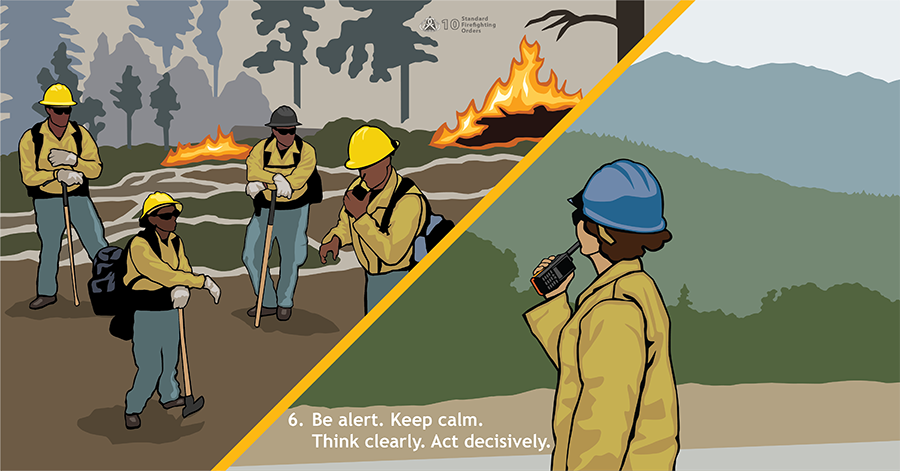
\includegraphics[width=0.49\textwidth, 
	trim={0cm 0cm 0cm 0cm}, 
	clip=true]
	{ops/pm110/110-06}	
	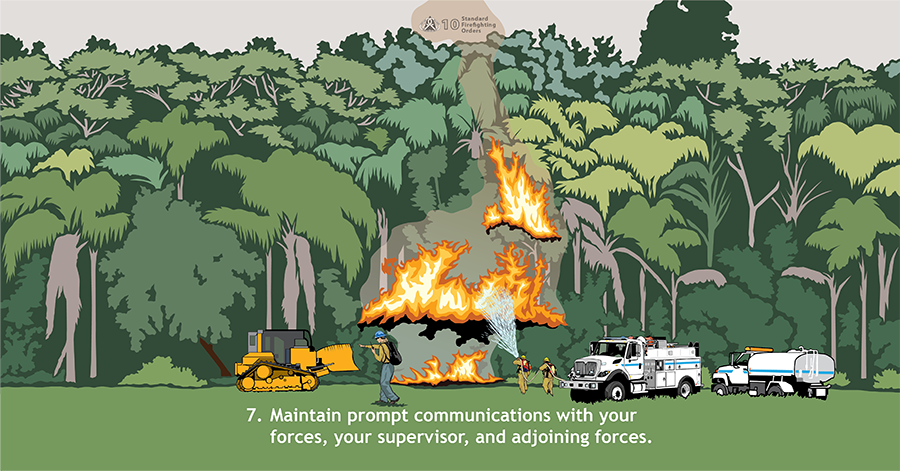
\includegraphics[width=0.49\textwidth, 
	trim={0cm 0cm 0cm 0cm}, 
	clip=true]
	{ops/pm110/110-07}
	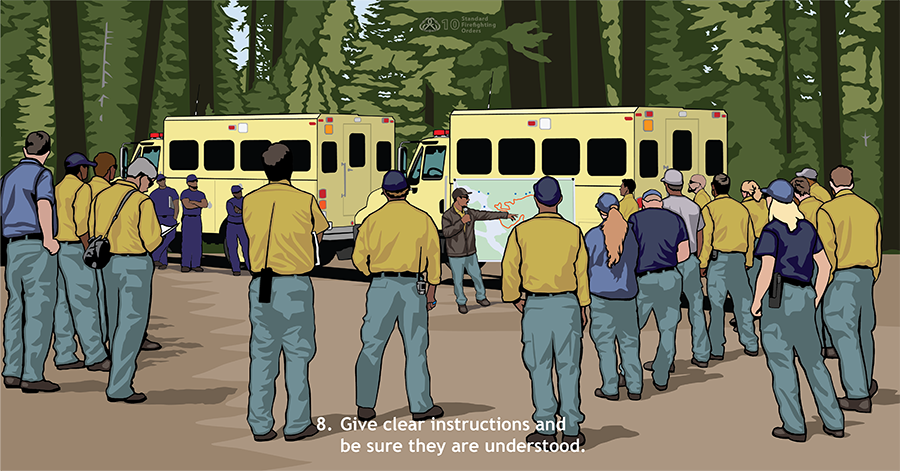
\includegraphics[width=0.49\textwidth, 
	trim={0cm 0cm 0cm 0cm}, 
	clip=true]
	{ops/pm110/110-08}	
	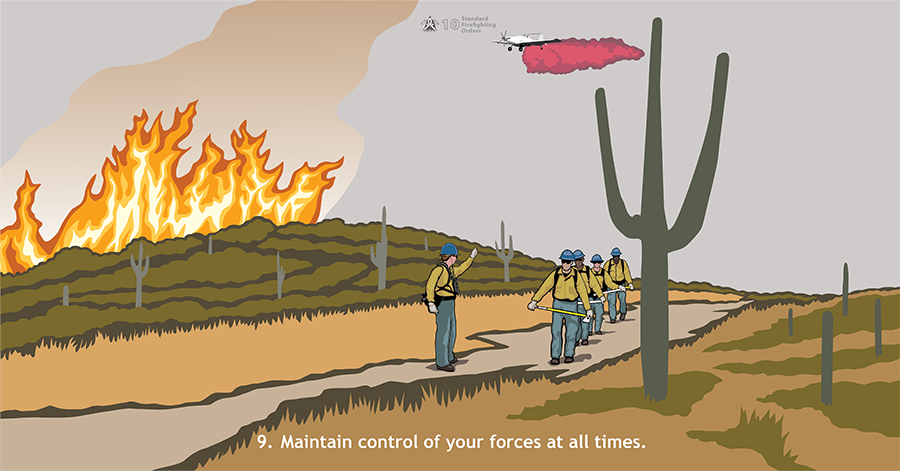
\includegraphics[width=0.49\textwidth, 
	trim={0cm 0cm 0cm 0cm}, 
	clip=true]
	{ops/pm110/110-09}
	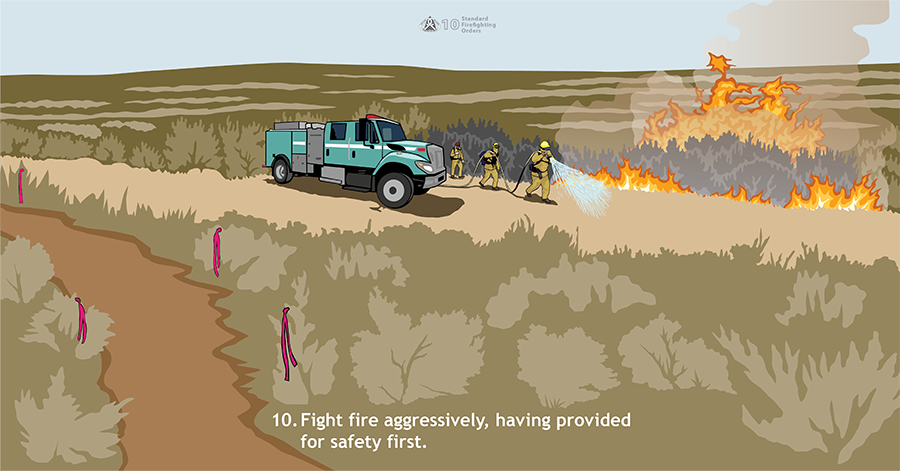
\includegraphics[width=0.49\textwidth, 
	trim={0cm 0cm 0cm 0cm}, 
	clip=true]
	{ops/pm110/110-10}
\end{minipage}



	
%\restoregeometry

